\centerline{\bf \Huge Домашнее задание.}
\centerline{\bf \Huge Задачи на разрезания I}

\begin{flushright}
        \scriptsize{20:31 прибыл Годжу Сатору}
\end{flushright}

\textit{Больше правильных вариантов разрезания на уникальные части = Больше баллов}

\problem{1}
Разрежьте фигуру на две равные части так, чтобы линия разреза шла по сторонам квадратов.

\begin{center}
    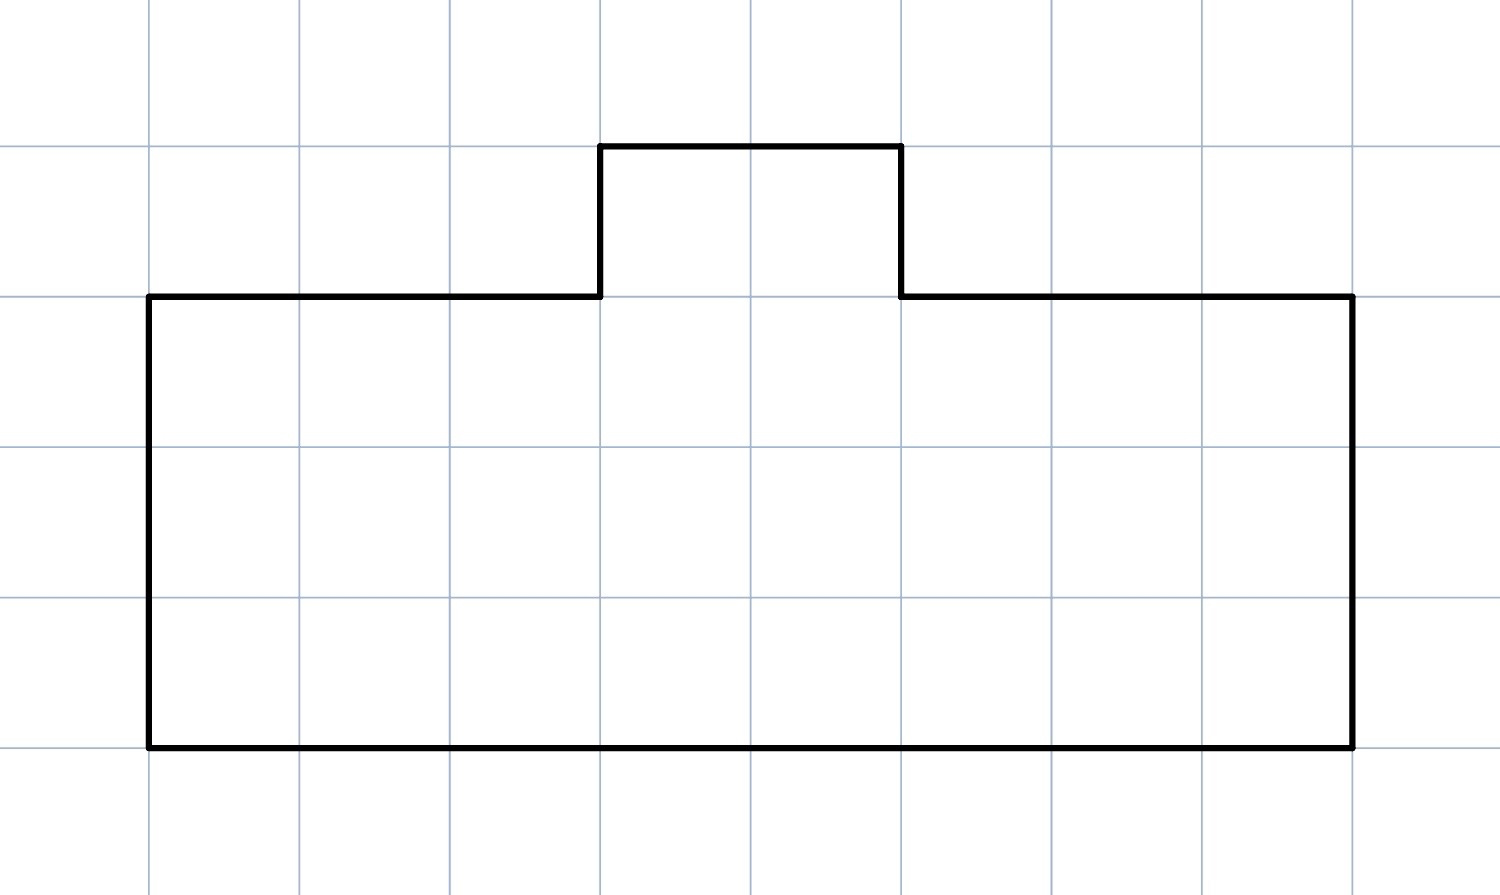
\includegraphics[width=0.2\textwidth]{ЭлМШ 2024-2025/I блок/Шиншиллы/HW_Cut_1.png}
\end{center}

\problem{2}
Разрежьте фигуру (с дыркой) на две равные части так, чтобы линия разреза шла по сторонам квадратов

\begin{center}
    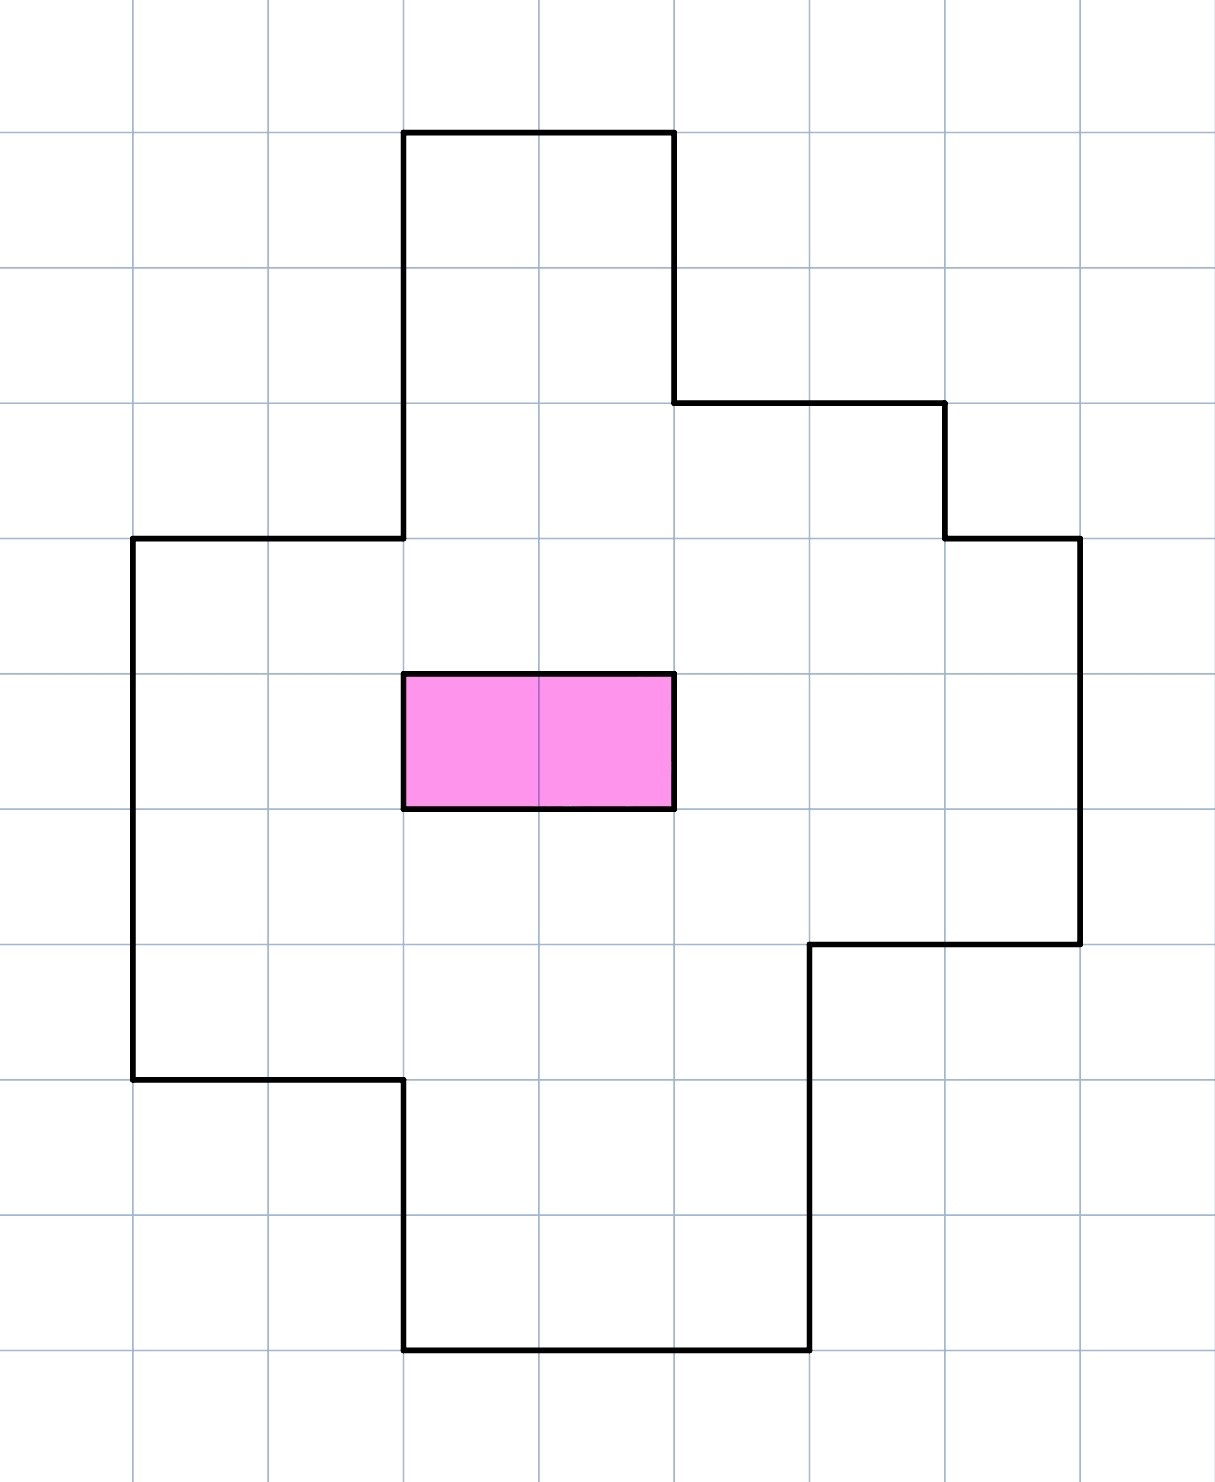
\includegraphics[width=0.2\textwidth]{ЭлМШ 2024-2025/I блок/Шиншиллы/HW_Cut_2.png}
\end{center}


\begin{wrapfigure}{r}{0.2\linewidth}
    \vspace{-15mm}
    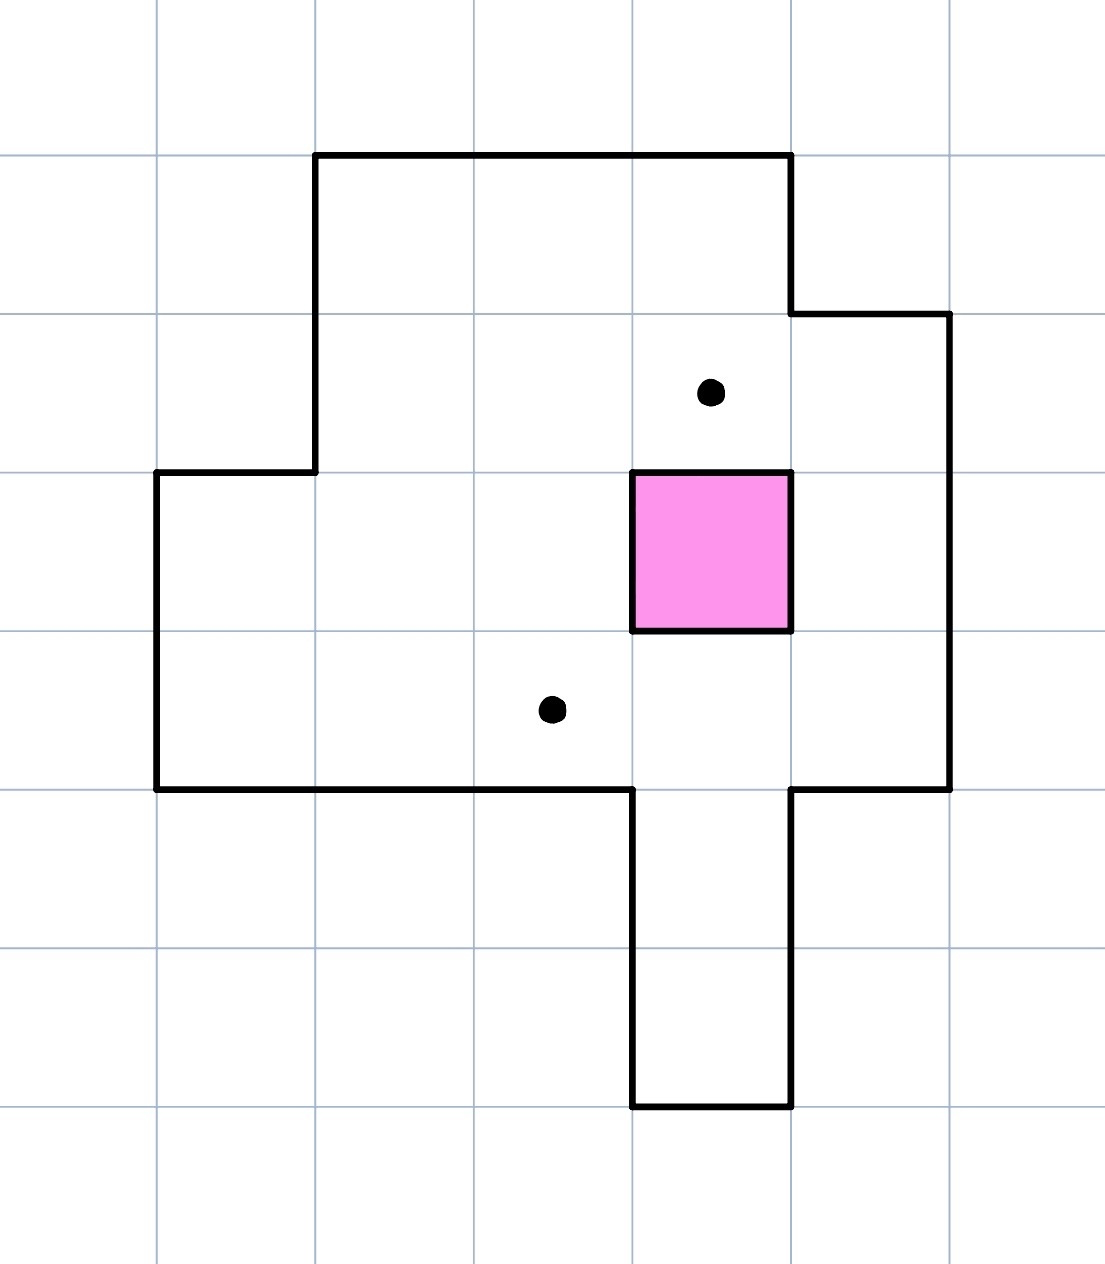
\includegraphics[width=\linewidth]{ЭлМШ 2024-2025/I блок/Шиншиллы/HW_Cut_3.png}
\end{wrapfigure}

\problem{3}
Разрежьте фигуру (с дыркой) на две равные части так, чтобы линия разреза шла по сторонам квадратов. Причем в каждой из частей должна быть одна точка.

\hspace{3mm}

\problem{4}
Разрежьте фигуру на четыре равные части так, чтобы линия разреза шла по сторонам квадратов.

\begin{center}
    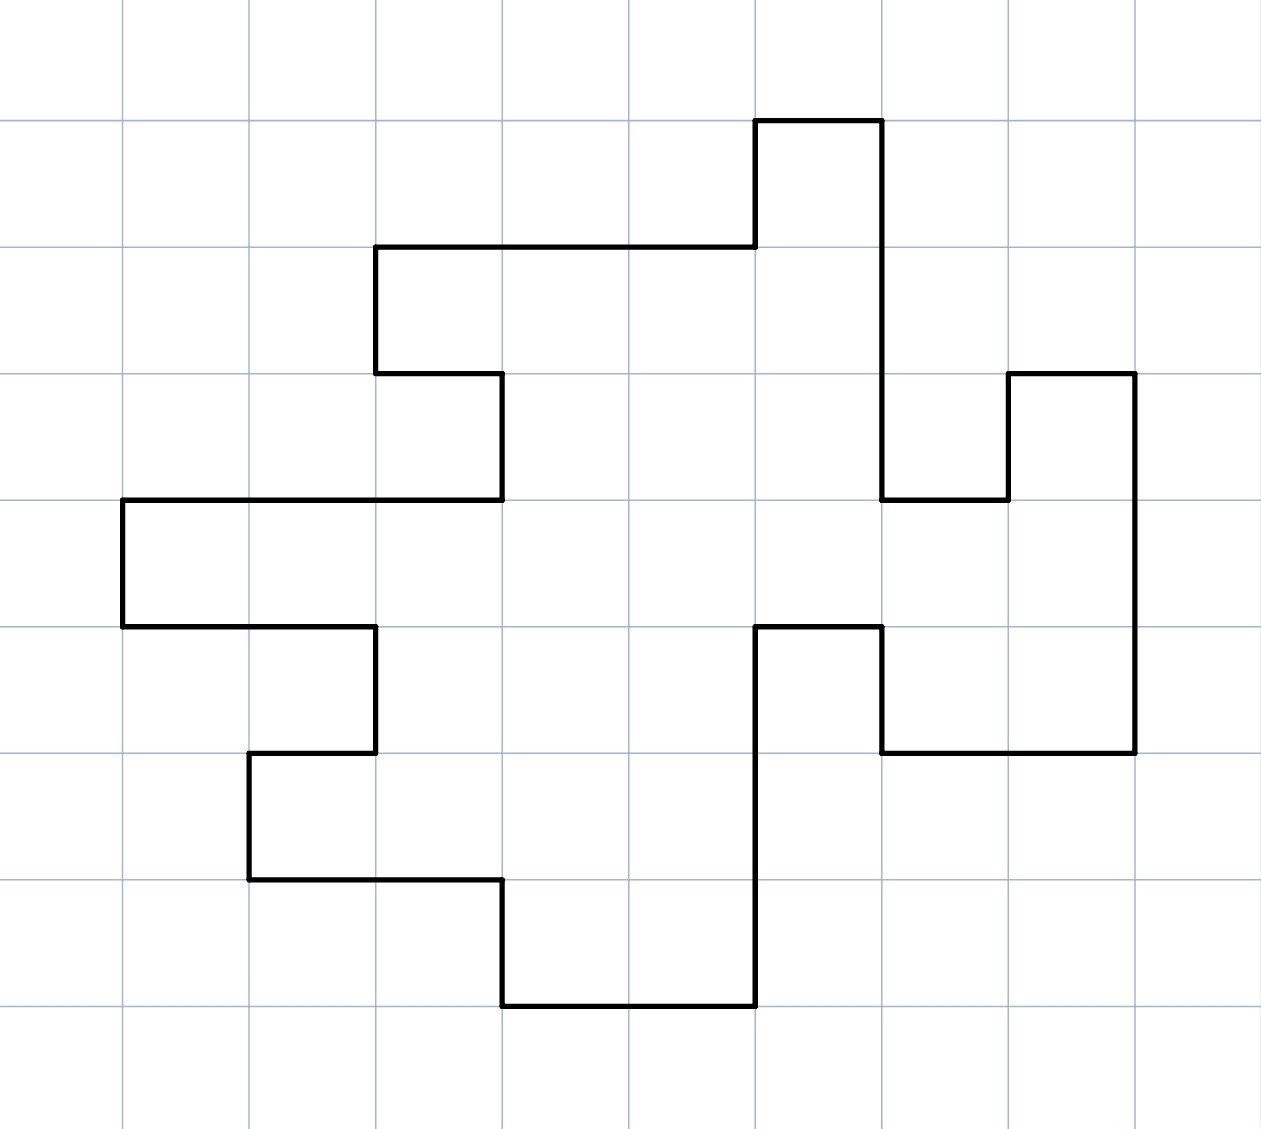
\includegraphics[width=0.2\textwidth]{ЭлМШ 2024-2025/I блок/Шиншиллы/HW_Cut_4.png}
\end{center}
